\documentclass[16pt]{scrreprt}
\usepackage[mathletters]{ucs}
\usepackage[utf8x]{inputenc}
\usepackage{amssymb}
\usepackage{amsmath}
\usepackage[usenames]{color}
\usepackage{hyperref}
\usepackage{wasysym}
\usepackage{graphicx}
\usepackage[normalem]{ulem}
\usepackage{enumerate}

\usepackage{listings}

\textwidth=15 cm
\linespread{1.5}

\lstset{ %
basicstyle=\footnotesize,       % the size of the fonts that are used for the code
showspaces=false,               % show spaces adding particular underscores
showstringspaces=false,         % underline spaces within strings
showtabs=false,                 % show tabs within strings adding particular underscores
frame=single,                   % adds a frame around the code
tabsize=2,                      % sets default tabsize to 2 spaces
breaklines=true,                % sets automatic line breaking
breakatwhitespace=false,        % sets if automatic breaks should only happen at whitespace
}




\title{Áramkörök}
\date{Sunday 03 March 2013}
\author{}

\begin{document}

\maketitle

\section{Áramköri elemek}

A készletben sokféle áramköri elemet fogsz találni. Néhányat már ismersz, néhány viszont még új lesz. Azért, hogy mindig meg tudd nézni, hogy melyik mit csinál, itt áttekintjük őket.

\subsubsection{Elem}

Úgy is hívják, hogy áramforrás, mert ez táplálja az áramot az áramkörbe. A te játékodban egy 9 voltos elemet találsz. Azért, hogy ne kelljen mindig újat venni, egy újratölthetőt tettünk bele. Viszont, ha szeretnéd, akkor tápegységet is használhatsz. Ez ugyanazt a szerepet játssza, mint az elem. 



Az áramkörben az elem negatív pólusából a pozitív felé haladnak az elektronok, és ez hajtja a ledeket, motorokat, csipogókat, villanykörtéket, és így tovább. 

Az elem jele a rajzokon ez lesz

\textbf{Rajz.}

\subsubsection{Kapcsolók}

A kapcsolókat arra vannak, hogy úgy szakíthassuk meg az áramkört, hogy azt ne kelljen szétszedni. Minden kapcsoló tulajdonképpen két drótból áll, amelyek összeérnek, ha a kapcsoló zárva van, és nem érnek össze, ha a kapcsoló nyitva van. Ha a kapcsoló zárva van, az elektronok szabadon tudnak áramlani az áramkörbe, viszont, ha a kapcsoló nyitva van, akkor nem történik semmi: az elektronok nem tudnak egyik helyről a másikra menni. 

Többféle kapcsolót is találsz majd. Lesz majd pillanatkapcsoló, ami csak akkor vezeti az áramot, ha megnyomod, olyan kapcsoló, amely bekapcsolt állapotban marad miután megnyomtad, illetve találsz majd olyat is, amelyik az áramkör két ága között "vált". Mindegyik mást célt szolgál, de a legegyszerűbben úgy érted meg a működésüket, ha kipróbálod őket.

A háromféle kapcsolót a következőképpen fogjuk jelölni:

Pillanatkapcsoló

\textbf{Rajz.}

Állandó kapcsoló

\textbf{Rajz.}

Váltó kapcsoló

\textbf{Rajz.}

\subsubsection{LED}

Ez tulajdonképpen ugyanazt csinálja, mint egy villanykörte, azaz világít, ha áramot kapcsolunk rá, azzal a különbséggel, hogy itt figyelni kell a polaritásra: ha fordítva teszed az áramkörbe, semmi nem fog történni. Próbáld csak ki! Ez egyébként azért van, mert a villanykörtével ellentétben, ahol egy izzó fémszál adja a fényt, a led egy félvezető eszköz, amely csak az egyik irányban vezeti az áramot. A másik irányban nemcsak, hogy nem világít, hanem úgy viselkedik, mint egy kikapcsolt kapcsoló. 



A készletedben mindegyik lednek van egy piros, és egy fekete lába. A pirosnak kell az elem pozitív pólusához csatlakozni. A ledek jele 

\textbf{Rajz.}



\subsubsection{Csipogó}

Ez egy nagyon egyszerű hangszóró, amely csak sípoló hangokat képes adni, de például beszédet nem lehet vele generálni. Ugyanúgy, ahogy a led, ez is csak egyféleképpen helyezhető az áramkörbe, mert polaritása van.

A csipogó jele

\textbf{Rajz.}



\subsubsection{Ellenállás}

Az ellenállás az áramkörben folyó áram nagyságának szabályozására szolgál. Nagyobb ellenállás jobban akadályozza az elektronok mozgását, ezért az áramkörben folyó áram kisebb lesz. Ez megmutatkozik például abban, hogy az ellenállással sorba kapcsolt led nem világít olyan fényesen. Az ellenállásokra rá lesz írva az értékük.

Az ellenállás jele

\textbf{Rajz.}



\subsubsection{Potenciométer}

Ez ugyanolyan, mint az ellenállás, csak egy gomb csavarásával (néha egy gomb elcsúsztatásával) az ellenállás nagysága változtatható. Ilyen potenciométereket találhatsz például a rádió hangerő-szabályozójában. 

A potenciométer jele

\textbf{Rajz.}



\subsubsection{Kondenzátor}

A kondenzátor nagyon hasonlít egy pici feltölthető elemhez: ha elektronokkal feltöltjük, akkor rövid ideig képes az áramkört táplálni. Viszont ez az idő rendszerint meglehetősen rövid, ezért a kondenzátort általában nem használják elem helyett. Ugyanakkor, a feltöltéshez szükséges időt mérésként lehet alkalmazni. Ezt fogjuk kipróbálni néhány csipogós és villogós áramkörben. A kondenzátorokra rá lesz írva a kapacitásuk, az, hogy mennyi elektront képesek tárolni. Minél nagyobb ez a szám, annál több elektron fér el a kondenzátorban, de annál hosszabb ideig tart feltölteni.

A kondenzátor jele

\textbf{Rajz.}



\subsubsection{Integrált áramkör}

A készletedben lesz egy integrált áramkör is. Ez általában egy kis fekete bigyó, amiben egy teljes áramkör van, csak olyan kicsi, hogy nem látjuk. Ezt fogjuk csipogók és villogók hajtására használni. 

Az integrált áramkör jele

\textbf{Rajz.}



\subsubsection{Áramköri lap}

Ez az, ahol az áramköröket felépíted. Ez nagyjából olyan, mint a LEGO-dban a zöld lap, amire különböző elemeket helyezhetsz. Itt minden áramköri elemnek lesz helye, és ezeket vezetékekkel tudod csatlakoztatni. 

\includegraphics[]{/home/v923z/useful/electro/andris/board.pdf}

\section{Áramkörök}

\subsubsection{Egyszerű ledes áramkör}

Most azt fogjuk kipróbálni, hogy a led mikor világít, és mikor nem. Ha a ledet egyszerűen az elem pozitív pólusához csatlakoztatod, akkor világít, ha viszont fordítva, akkor nem. 

\textbf{Rajz.} Lehet párhuzamos kapcsolás is.

Azt is kipróbálhatod, hogy ha két ledet sorba kapcsolsz úgy, hogy a polaritásaik egymással ellentétesek, akkor nem folyik áram az áramkörben, egyik led sem világít.

\textbf{Rajz.}

Azt is kipróbálhatod, hogy mi történik, ha a leddel sorba kötsz egy ellenállást: ha túl nagy ellenállást választasz, a led olyan halványan fog világítani, hogy nem is látod. 

\subsubsection{Közlekedési lámpa}

Néhány leddel, és néhány kapcsolóval egyszerűen építhetsz egy közlekedési lámpát. A ledeket párhuzamosan kell kapcsolni, hogy ne egyszerre világítsanak. 

\textbf{Rajz.}

\subsubsection{Villogó}

A következő áramkör egy egyszerű villogó: A led ki-be kapcsol. A ki-be kapcsolás sebességét az ellenállások és a kondenzátorok nagysága határozza meg. Kipróbálhatód, hogy mi történik, ha kisebb, vagy nagyobb ellenállásokat, vagy kondenzátorokat teszel az áramkörbe. Előfordulhat, hogy ha túl kis ellenállással vagy kondenzátorral próbálkozol, akkor a villogó olyan gyors lesz, hogy nem is látod a villogást.

\includegraphics[]{/home/v923z/useful/electro/andris/astable_555.pdf}

Ha két ledet sorba kötsz úgy, ahogy a rajzon látod, akkor ezek felváltva fognak világítani.

\includegraphics[]{/home/v923z/useful/electro/andris/astable_555b.pdf}

\textbf{Rajz.}

\subsubsection{Változtatható villogó}

Ez az áramkör nagyon hasonló az előzőhöz, azzal a különbséggel, hogy most a villogás sebességét változtatni lehet. Ezért az egyik ellenállást kicseréljük egy potenciométerre.

\textbf{Rajz.}

\subsubsection{Csipogó}

Ez az áramkör nagyon hasonló a villogós áramkörre, de most a led helyett egy csipogót használunk. Arra is figyelni kell, hogy mivel a hangoknak a frekvenciája (az, hogy milyen gyorsan rezeg) sokkal magasabb, mint ami a villogónál volt, ezért most kisebb ellenállásokat és kisebb kondenzátorokat kell használnunk. 

\includegraphics[]{/home/v923z/useful/electro/andris/beeper_555.pdf}

\subsubsection{Változtatható csipogó}

Ahogy a villogónál, itt is, ha az egyik ellenállást kicseréljük egy potenciométerre, a csipogás frekvenciája változtatható lesz. 

\textbf{Rajz.}

\subsubsection{Kéthangú csipogó}

Ez az áramkör két frekvencián fog szólni, attól függően, hogy megnyomod-e a pillanatkapcsolót, vagy nem. Ez azon alapul, hogy a pillanatkapcsoló megnyomásakor a második ellenállást párhuzamosan kapcsoljuk az elsővel, és ez csökkenti az úgynevezett eredő ellenállást.

\textbf{Rajz.}

\subsubsection{Kéthangú csipogó másképpen (sziréna)}

Ez az áramkör is két frekvencián fog szólni, de most nem kell megnyomnod egy kapcsolót, hanem automatikusan változik a két hang. Ez nagyon hasonló a rendőrautó szirénájához. Itt két áramkört kell összeépíteni: egy csipogót, és egy villogót. A két áramkört egyetlen vezetékkel kell összekötni. Ez fogja a hang frekvenciáját meghatározni. 

\includegraphics[width=0.95\textwidth]{/home/v923z/useful/electro/andris/siren_555.pdf}


\subsubsection{Szaggatott csipogó}

Most egy olyan áramkört fogunk építeni, ami néha csipog, néha nem. Ehhez megint két áramkört kell összerakni: egy csipogót, és egy villogót, tehát nagyon hasonló, ahhoz, amit a kéthangú csipogóval csináltál. A két áramkört egyetlen vezetékkel kell összekötni. Amikor a feszültség ezen a vezetéken magas (amikor a LED világít), akkor a csipogó sípol, amikor pedig alacsony (ilyenkor a LED kialszik), akkor a csipogó nem ad hangot.  

\includegraphics[width=0.95\textwidth]{/home/v923z/useful/electro/andris/temporary_beeper_555.pdf}

\subsubsection{Futófény}

A következő áramkörökkel futófényt fogunk készíteni. Az áramkörök nagyon hasonlóak: mindegyikben van egy egység,
amelyik az órajelet generálja. Ez az egység ugyanaz az áramkör, mint amit a villogóban, vagy a csipogóban már láttál.
Annak az egységnek a kimenetét, a hármas lábat, nem ledhez fogjuk csatlakoztatni, hanem egy másik integrált áramkörhöz.
Ez az egység csatlakozik majd a ledekhez. Csak az elsőnél rajzolom le az egész áramkört, a többinél már csak a ledes
egységet. Az órajel-generátort ugyanúgy kell megcsinálni.

\subsubsection{Futófény három leddel}
\includegraphics[width=0.95\textwidth]{/home/v923z/useful/electro/andris/runninglight_3.pdf}

\subsubsection{Futófény négy leddel}
\includegraphics[width=0.95\textwidth]{/home/v923z/useful/electro/andris/runninglight_4b.pdf}

\subsubsection{Futófény öt leddel}
\includegraphics[width=0.95\textwidth]{/home/v923z/useful/electro/andris/runninglight_5b.pdf}

\subsubsection{Futófény hat leddel}
\includegraphics[width=0.95\textwidth]{/home/v923z/useful/electro/andris/runninglight_6.pdf}

\subsubsection{Futófény hét leddel}
\includegraphics[width=0.95\textwidth]{/home/v923z/useful/electro/andris/runninglight_7.pdf}

\subsubsection{Futófény nyolc leddel}
\includegraphics[width=0.95\textwidth]{/home/v923z/useful/electro/andris/runninglight_8.pdf}

\subsubsection{Futófény kilenc leddel}
\includegraphics[width=0.95\textwidth]{/home/v923z/useful/electro/andris/runninglight_9.pdf}

\subsubsection{Futófény tíz leddel}
\includegraphics[width=0.95\textwidth]{/home/v923z/useful/electro/andris/runninglight_10.pdf}

\subsubsection{Futófény sötét futóval}
A következő áramkör nagyon hasonló a közönséges futófényhez, azzal a különbséggel, hogy most négy led fog égni, és
mindig csak egy lesz sötét. 

\includegraphics[width=0.95\textwidth]{/home/v923z/useful/electro/andris/runningdarkness_5.pdf}

\subsubsection{Futófény sötét futóval vagy fényes futóval}
Most még egy fokkal bonyolultabbá tesszük az áramkört: a kapcsoló segítségével ki tudjuk választani, hogy sötét, vagy
világos legyen-e a futó. A különbség az előző áramkörökhöz képest annyi, hogy még egy kapcsolót is be kell építenünk,
és a kapcsoló egyik végét a pozitív, a másikat pedig a negatív feszültséghez kell csatlakoztatnunk. A kapcsoló középső
a két ledsorhoz kapcsolódik. 

\includegraphics[width=0.95\textwidth]{/home/v923z/useful/electro/andris/runningdarkness_switch.pdf}

\subsubsection{Liftlámpa}
Most két futófényt fogunk összekapcsolni úgy, hogy az eredmény olyan legyen, mint a liftajtó lámpája. Meg tudod
csinálni, hogy a másik irányba fussanak a fények?

\includegraphics[width=0.95\textwidth]{/home/v923z/useful/electro/andris/lift_light.pdf}

\subsubsection{Futófény még egyszer}
Most olyan futófényt fogunk építeni, amelyik oda-vissza fut, de nem úgy, mint a liftlámpa. Az eddig megismerteken kívül
szükségünk lesz még 10 diódára. A dióda csak egy irányban engedi folyni az áramot. Ha megnézed az áramkörödet, akkor az
egyik oldalon fekete csíkokat látsz. Vigyázz, hogy a fekete csík úgy álljon, mint ahogy az ábrán látod, egyébként semmi
nem fog történni. Viszont ha figyelmesed állítod össze az áramkört, meglátod, érdekes lesz!

\includegraphics[width=0.95\textwidth]{/home/v923z/useful/electro/andris/knightrider_5.pdf}

\end{document}
